\let\negmedspace\undefined
\let\negthickspace\undefined
\documentclass[journal]{IEEEtran}
\usepackage[a5paper, margin=10mm, onecolumn]{geometry}
%\usepackage{lmodern} % Ensure lmodern is loaded for pdflatex
\usepackage{tfrupee} % Include tfrupee package

\setlength{\headheight}{1cm} % Set the height of the header box
\setlength{\headsep}{0mm}     % Set the distance between the header box and the top of the text

\usepackage{gvv-book}
\usepackage{gvv}
\usepackage{cite}
\usepackage{amsmath,amssymb,amsfonts,amsthm}
\usepackage{algorithmic}
\usepackage{graphicx}
\usepackage{textcomp}
\usepackage{xcolor}
\usepackage{txfonts}
\usepackage{listings}
\usepackage{enumitem}
\usepackage{mathtools}
\usepackage{gensymb}
\usepackage{comment}
\usepackage[breaklinks=true]{hyperref}
\usepackage{tkz-euclide} 
\usepackage{listings}
% \usepackage{gvv}                                        
\def\inputGnumericTable{}                                 
\usepackage[latin1]{inputenc}                                
\usepackage{color}                                            
\usepackage{array}                                            
\usepackage{longtable}                                       
\usepackage{calc}                                             
\usepackage{multirow}                                         
\usepackage{hhline}                                           
\usepackage{ifthen}                                           
\usepackage{lscape}
\begin{document}

\bibliographystyle{IEEEtran}

\title{5.2.56}
\author{EE25BTECH11054 - S.Harsha Vardhan}
% \maketitle
% \newpage
% \bigskip
\maketitle 
\renewcommand{\thefigure}{\theenumi}
\renewcommand{\thetable}{\theenumi}
\setlength{\intextsep}{10pt} % Space between text and floats

\numberwithin{align}{enumi}
\numberwithin{figure}{enumi}
\renewcommand{\thetable}{\theenumi}
\vspace{-1em}
\textbf{Question}:\\
	Solve the following system of linear equations.
	\[
	\frac{5}{x-1} + \frac{1}{y-2} = 2 \quad
	\frac{6}{x-1} - \frac{3}{y-2} = 1
	\]
	
	\solution\\
	Let 
	\begin{align}
		u = \frac{1}{x-1}, \quad v = \frac{1}{y-2}.
	\end{align}
	The given system becomes a linear system in terms of $u$ and $v$:
	\begin{align}
		5u + v &= 2 \\
		6u - 3v &= 1
	\end{align}
	In matrix form, this is $\vec{A}\vec{x} = \vec{b}$, where:
	\begin{align}
		\myvec{5 & 1 \\ 6 & -3} \myvec{u \\ v} = \myvec{2 \\ 1}.
	\end{align}
	Let 
	\begin{align}
		\vec{A} = \myvec{5 & 1 \\ 6 & -3}, \quad \vec{b} = \myvec{2 \\ 1}.
	\end{align}
	We can solve this using Gauss-Jordan elimination on the augmented matrix $\myvec{\vec{A}|\vec{b}}$.
	\begin{align}
		\augvec{2}{1}{5 & 1 & 2 \\ 6 & -3 & 1}
		&\xrightarrow{R_1 \rightarrow \frac{1}{5}R_1}
		\augvec{2}{1}{1 & \frac{1}{5} & \frac{2}{5} \\ 6 & -3 & 1}
		\xrightarrow{R_2 \rightarrow R_2 - 6R_1}
		\augvec{2}{1}{1 & \frac{1}{5} & \frac{2}{5} \\ 0 & -\frac{21}{5} & -\frac{7}{5}} 
        \end{align}
        \begin{align}
		\augvec{2}{1}{1 & \frac{1}{5} & \frac{2}{5} \\ 0 & -\frac{21}{5} & -\frac{7}{5}}&\xrightarrow{R_2 \rightarrow -\frac{5}{21}R_2}
		\augvec{2}{1}{1 & \frac{1}{5} & \frac{2}{5} \\ 0 & 1 & \frac{1}{3}} 
		\xrightarrow{R_1 \rightarrow R_1 - \frac{1}{5}R_2}
		\augvec{2}{1}{1 & 0 & \frac{1}{3} \\ 0 & 1 & \frac{1}{3}}
	\end{align}
	From the reduced row echelon form, we have the solution for $u$ and $v$:
	\begin{align}
		\myvec{u \\ v} = \myvec{\frac{1}{3} \\ \frac{1}{3}}
	\end{align}
	Now, we back-substitute to find $x$ and $y$:
	\begin{align}
		u = \frac{1}{x-1} = \frac{1}{3} &\implies x - 1 = 3 \implies x = 4, \\
		v = \frac{1}{y-2} = \frac{1}{3} &\implies y - 2 = 3 \implies y = 5.
	\end{align}
	Thus, the final solution is:
	\begin{align}
		\myvec{x \\ y} = \myvec{4 \\ 5}.
	\end{align}
    \begin{figure}[h]
    \centering
    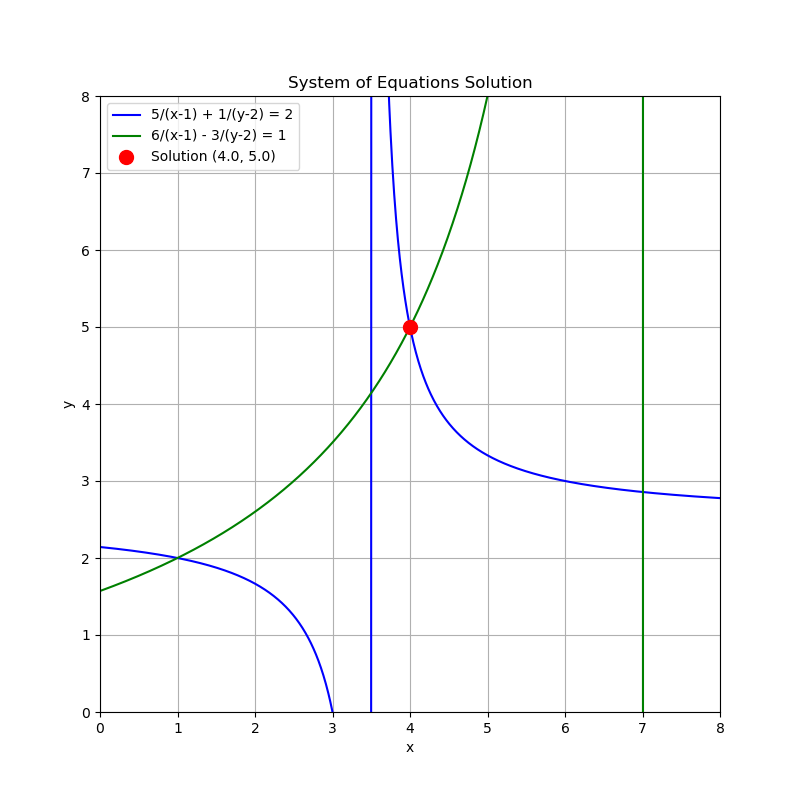
\includegraphics[width=1.1\linewidth]{figs/Figure_4.png}
    \caption{}
    \label{fig:placeholder}
\end{figure}
	
\end{document}